\documentclass{article}\usepackage[]{graphicx}\usepackage[]{color}
% maxwidth is the original width if it is less than linewidth
% otherwise use linewidth (to make sure the graphics do not exceed the margin)
\makeatletter
\def\maxwidth{ %
  \ifdim\Gin@nat@width>\linewidth
    \linewidth
  \else
    \Gin@nat@width
  \fi
}
\makeatother

\definecolor{fgcolor}{rgb}{0.345, 0.345, 0.345}
\newcommand{\hlnum}[1]{\textcolor[rgb]{0.686,0.059,0.569}{#1}}%
\newcommand{\hlstr}[1]{\textcolor[rgb]{0.192,0.494,0.8}{#1}}%
\newcommand{\hlcom}[1]{\textcolor[rgb]{0.678,0.584,0.686}{\textit{#1}}}%
\newcommand{\hlopt}[1]{\textcolor[rgb]{0,0,0}{#1}}%
\newcommand{\hlstd}[1]{\textcolor[rgb]{0.345,0.345,0.345}{#1}}%
\newcommand{\hlkwa}[1]{\textcolor[rgb]{0.161,0.373,0.58}{\textbf{#1}}}%
\newcommand{\hlkwb}[1]{\textcolor[rgb]{0.69,0.353,0.396}{#1}}%
\newcommand{\hlkwc}[1]{\textcolor[rgb]{0.333,0.667,0.333}{#1}}%
\newcommand{\hlkwd}[1]{\textcolor[rgb]{0.737,0.353,0.396}{\textbf{#1}}}%
\let\hlipl\hlkwb

\usepackage{framed}
\makeatletter
\newenvironment{kframe}{%
 \def\at@end@of@kframe{}%
 \ifinner\ifhmode%
  \def\at@end@of@kframe{\end{minipage}}%
  \begin{minipage}{\columnwidth}%
 \fi\fi%
 \def\FrameCommand##1{\hskip\@totalleftmargin \hskip-\fboxsep
 \colorbox{shadecolor}{##1}\hskip-\fboxsep
     % There is no \\@totalrightmargin, so:
     \hskip-\linewidth \hskip-\@totalleftmargin \hskip\columnwidth}%
 \MakeFramed {\advance\hsize-\width
   \@totalleftmargin\z@ \linewidth\hsize
   \@setminipage}}%
 {\par\unskip\endMakeFramed%
 \at@end@of@kframe}
\makeatother

\definecolor{shadecolor}{rgb}{.97, .97, .97}
\definecolor{messagecolor}{rgb}{0, 0, 0}
\definecolor{warningcolor}{rgb}{1, 0, 1}
\definecolor{errorcolor}{rgb}{1, 0, 0}
\newenvironment{knitrout}{}{} % an empty environment to be redefined in TeX

\usepackage{alltt}
\usepackage{Sweave}
\usepackage{float}
\usepackage{graphicx}
\usepackage{tabularx}
\usepackage{siunitx}
\usepackage{amssymb} % for math symbols
\usepackage{amsmath} % for aligning equations
\usepackage{textcomp}
\usepackage{mdframed}
\usepackage[T1]{fontenc}
\usepackage{subcaption}
\usepackage{natbib}
\bibliographystyle{..//refs/styles/besjournals.bst}
\usepackage[small]{caption}
\setlength{\captionmargin}{30pt}
\setlength{\abovecaptionskip}{0pt}
\setlength{\belowcaptionskip}{10pt}
\captionsetup{justification=raggedright,singlelinecheck=false}
\topmargin -1.5cm        
\oddsidemargin -0.04cm   
\evensidemargin -0.04cm
\textwidth 16.59cm
\textheight 21.94cm 
%\pagestyle{empty} %comment if want page numbers
\parskip 7.2pt
\renewcommand{\baselinestretch}{1.5}
\parindent 0pt
%\usepackage{lineno}
%\linenumbers

%cross referencing:
\usepackage{xr}
\usepackage{xr-hyper}
\externaldocument{/Users/CatherineChamberlain/Documents/git/microclimates/docs/micro_supp}

\newmdenv[
  topline=true,
  bottomline=true,
  skipabove=\topsep,
  skipbelow=\topsep
]{siderules}
\IfFileExists{upquote.sty}{\usepackage{upquote}}{}
\begin{document}

\noindent\textbf{\Large{Understanding growing degree days to predict spring phenology under climate change}}

\noindent Authors:\\
C. J. Chamberlain $^{1,2}$ \& E. M. Wolkovich $^{1,2,3}$
\vspace{2ex}\\
\emph{Author affiliations:}\\
$^{1}$Arnold Arboretum of Harvard University, 1300 Centre Street, Boston, Massachusetts, USA; \\
$^{2}$Organismic \& Evolutionary Biology, Harvard University, 26 Oxford Street, Cambridge, Massachusetts, USA; \\
$^{3}$Forest \& Conservation Sciences, Faculty of Forestry, University of British Columbia, 2424 Main Mall, Vancouver, BC V6T 1Z4\\
\vspace{2ex}
$^*$Corresponding author: 248.953.0189; cchamberlain@g.harvard.edu\\

\renewcommand{\thetable}{\arabic{table}}
\renewcommand{\thefigure}{\arabic{figure}}
\renewcommand{\labelitemi}{$-$}
\setkeys{Gin}{width=0.8\textwidth}

%%%%%%%%%%%%%%%%%%%%%%%%%%%%%%%%%%%%%%%%%%%%%%%
%%%%%%%%%%%%%%%%%%%%%%%%%%%%%%%%%%%%%%%%%%%%%%%


\section*{Introduction}
\begin{enumerate}
\item In ecology, we have the fundamental issue of understanding and applying methods to accurately predict shifts in climate and the broader impacts of these shifts.
  \begin{enumerate}
  \item Often we use mixed models to answer ecological questions, though we do not always understand the intricacies of the model output, nor do we investigate what is missing from the model output.
  \item Here, we work to understand mixed models using simulation data and test myriad hypotheses through these simulations. 
  \item These methods can be applied to many ecological questions investigating climate data across global habitats but here we will investigate the effects of climate measurements and site on spring plant phenology. 
  \end{enumerate}
  
\item Understanding and predicting plant phenology in temperate deciduous forests is critical as it both shapes community structure and also influences major ecosystem services such as resource and forest management. 
  \begin{enumerate} 
  \item Climate change and urbanization are advancing spring timing---such as budburst and leafout, which  are strongly cued by temperature, resulting in longer growing seasons \citep{Chuine2001} which ultimately impacts these services.  
  \item Temperate forests sequester carbon and help mitigate the negative effects of climate change and---with earlier spring phenology and longer growing seasons---there has been an increase in carbon uptake \citep{Keenan2014}.
  \item But our understanding of how climate change is impacting this timing of spring is incomplete, especially in urban versus natural forest habitats. 
  \end{enumerate}
  
\item Urbanization has led to the formation of urban heat islands, which have been shown to affect plant phenology and lead to earlier spring leafout \citep{Meng2020}. 
  \begin{enumerate}
  \item These trends are crucial to understand in order to predict plant development with warming. 
  \item Tracking heat accumulation is one way to measure and forecast spring leafout, which is often predicted through the growing degree day (GDD) model \citep{Cook2012,Crimmins2020,Phillimore2013,Schwartz2006,Vitasse2011}.
  \item The GDD model simply sums temperatures above a certain threshold---ideally around 0$^{\circ$C as estimates are proven to be more accurate \citep{Man2010}---and different species often require a different number of GDDs to leaf out. 
  \item GDDs accumulate at a faster rate when mean temperatures are higher, thus different sites or different climate measurement methods may record different GDD thresholds for leafout. 
  \item Spring leafout timing can have cascading effects to pollinators \citep{Boggs2012, Pardee2017}, on carbon dynamics \citep{Richardson2013} and albedo \citep{Williamson2016}, thus integrating the growing degree day model successfully is essential for predicting the effects of climate change on temperate systems. 
  \end{enumerate}

\item Phenology is often measured through satellite, remote sensing or PhenoCam images to detect spring `green-up' \citep{Meng2020, Liu2018, Richardson2015} but these methods fail to detect the species---or even site-level---nuances in leafout timing \citep{Elmendorf2019}.
  \begin{enumerate}
  \item Intensive, on the ground observations of individual budburst and leafout timing is the most effective way to implement new methods in calculating growing degree days and predicting future phenology. 
  \item Urban environments additionally provide a natural laboratory for assessing the effects of warming on temperate tree and shrub species as these sites are warming at a faster rate than more rural habitats \citep{Pickett2011, Grimm2008}.
  \end{enumerate}
  
\item Arboreta and botanical gardens offer a unique lens to investigate climate change and local adaptation studies by incorporating varying seed sources---or provenance locations---thus they mimic common garden experiments \citep{Primack2009}. 
  \begin{enumerate}
  \item Most arboreta keep diligent acquisition records, providing visitors and scientists information on seed sources and tree age \citep{Dosmann2006}, whereas in forests, tree cores must be assessed to get as accurate an estimate on tree age and there is no variation in provenance location.
  \end{enumerate}
  
\item As GDD is a predominant indicator of spring phenology, having accurate and consistent weather data is essential for better estimates of budburst or leafout, especially with warming.
  \begin{enumerate}
  \item To facilitate scaling and minimize error due to microclimatic effects, researchers often deploy standalone weather loggers---such as HOBO sensors---which may provide higher resolution weather data \citep{Schwartz2013a,Whiteman2000}.
  \item Though deploying temperature loggers is not always feasible, especially when investigating large spatiotemporal shifts in GDDs. 
  \end{enumerate}
  
\item Here, we use both simulations, models and real data to test our hypotheses on modeling GDD accuracy in a warming world and conclude with a series of simulated forecasts to estimate changes in GDD estimates.
  \begin{enumerate}
  \item Our major hypotheses are as follows...
  \item Weather stations are less accurate measures of the same weather than hobo loggers.
  \item Urban environments require fewer GDDs to leafout than forest habitats.
  \item Individuals with provenance latitudes from more northern locations require fewer GDDs to leafout. 
  \item Weather stations will record warmer temperatures at urban sites and cooler temperatures at forest sites compared to hobo loggers. 
  \end{enumerate}
\end{enumerate}
  

\section*{Methods}
\subsection*{Sites}
\begin{enumerate}
\item We chose two sites---one urban arboretum and one forest---with overlapping species and climates to compare the number of growing degree days to leafout across species. 
  \begin{enumerate}
  \item The urban site is in Boston, MA at the Arnold Arboretum of Harvard University (42$^{\circ}$17' N -71$^{\circ}$8' W).
  \item The Arnold Arboretum is 281 acres and contains 3825 woody plant taxa from North America, Europe and Asia.
  \item The forest site is in Petersham, MA at the Harvard Forest (42$^{\circ}$31'53.5' N -72$^{\circ}$11'24.1' W).
  \item The Harvard Forest is 1446 acres and has a range of elevation of 220-410m. 
  \end{enumerate}
\end{enumerate}

\subsection*{Simulations} %%% I may have to reorder this a bit to end up following the direction we want to convey. 
%% The new order may be... 1) weather stations are more noisy, 2) urban environments require fewer GDDs, 3) weather stations will record different weather across different sites, 3) provenance stuffs
\begin{enumerate}
\item We simulate test data in order to test our hypotheses and assess the model output results. 
  \begin{enumerate}
  \item In order to exhaustively examine all hypotheses, we build our simulation data to address very simple to more complex questions.
  \item We first start by examining what the model output would look like if we just make the weather station data less accurate.
  \item To do this, we create an effect of method on our GDD threshold value and then increase error on the weather station measurements by increasing the sigma value for our random distribution creation (see Supplemental information on Data Simulation). 
  \item Next, we incorporate climate data by again establishing a random distribution around a mean temperature for each site and then add noise to this weather data to create ``microclimatic'' effects. 
  \item Using this climate data, we then find the day of budburst when the unique GDD threshold is reached for each individual. 
  \item For the following hypothesis testing urban effect, we create simulation data that manipulates the GDD threshold for the urban versus forest sites by lowering the GDD threshold for individuals at the arboretum. 
  \item Next, we apply the same ``microclimatic effect'' as above to test microclimatic variation across the two sites. 
  \item We repeat these steps for the provenance latitude hypothesis by having individuals from more northern provenances requiring fewer GDDS and then apply the ``microclimatic effect''.
  \end{enumerate}
\end{enumerate}

\subsection*{Real Data}
\begin{enumerate}
\item Phenology observations across the Arnold Arboretum were collected by trained citizen scientists from the Tree Spotters National Phenology Network program \citep{USA-NPN2016}. 
  \begin{enumerate}
  \item The Tree Spotter volunteers observed 15 tree and shrub species---ranging from early-budbursting to late-budbursting---and each species had 5 individuals for a total of 75 trees.
  \item Species included in the study were \textit{Acer saccharum}, \textit{Acer rubrum}, \textit{Aesculus flava}, \textit{Betula nigra}, \textit{Betula alleghaniensis}, \textit{Carya glabra}, \textit{Carya ovata}, \textit{Fagus grandifolia}, \textit{Hamamelis virginiana}, \textit{Populus deltoides}, \textit{Quercus alba}, \textit{Quercus rubra}, \textit{Tilia amaericana}, \textit{Vaccinium corymbosum}, and \textit{Viburnum nudum} (Figure \ref{fig:phylo}).  
  \item In September 2018, we placed 15 hobo loggers around the Tree Spotter route to compare hobo logger temperatures to the weather station temperatures recorded. 
  \item We then used budburst observations for each individual and calculated GDDs until budburst starting from 15 February using both the hobo logger data and then the weather station data. 
  \end{enumerate}

\item Phenology observations for the Harvard Forest have been collected by Dr John O'Keefe since 1990 \citep{OKeefe2014} along the Prospect Hill Tract. 
  \begin{enumerate}
  \item Species observed by Dr John O'Keefe include \textit{Acer saccharum}, \textit{Acer rubrum}, \textit{Acer pensylvanicum}, \textit{Betula alleghaniensis}, \textit{Fagus grandifolia}, \textit{Fraxinus americana}, \textit{Hamamelis virginiana}, \textit{Quercus alba} and \textit{Quercus rubra} (Figure \ref{fig:phylo}).
  \item The same methods were applied at the Harvard Forest where we placed 15 hobo loggers at regular intervals along the Prospect Hill Tract, calculated GDD estimates from 15 February 2019 until budburst for each individual using hobo logger data and then weather station data. 
  \end{enumerate}
\end{enumerate}
  
\subsection*{Forecasting}
\begin{enumerate}
\item Using simulated data, we tested GDD accuracy across various GDD threshold requirements with warming of 1$^{\circ$C to 10$^{\circ$C. 
  \begin{enumerate}
  \item We also evaluate accuracy using different base temperatures for calculating GDD (i.e., -5$^{\circ$C, 0$^{\circ$C, 5$^{\circ$C and 10$^{\circ$C).
  \end{enumerate}
\end{enumerate}

\subsection*{Shiny App}
\begin{enumerate}
\item To show the above simulations, real data and forecasts in one location we use a Shiny Application. 
  \begin{enumerate}
  \item Using the R package `shiny' \citep{shiny2021}, version 1.6.0, we developed a Shiny App that contains five pages: (1) `Home' which has information on the application, (2) `Hypothesis Testing' which runs the simulation data and allows users to manipulate the inputs, (3) `Simulation Data for Model Testing' which runs simulation data to test the model and make sure the model outputs are accurate, (4) `Real Data and Analyze Results' which uses real data and runs analyses to be used to compare to the `Hypothesis Testing' output and (5) `Forecasting GDD with Warming' which forecasts GDD accuracy under warming. 
  \item The Shiny App is meant for users to understand our suggested approach to model testing and interpreting mixed model results. 
  \end{enumerate}
\end{enumerate}

\subsection*{Data analysis}
\begin{enumerate}
\item Using Bayesian hierarchical models with the rstan package \citep{rstan2019}, version 2.19.2,  in R \citep{R}, version 3.3.1, we estimated the effects of urban or provenance effect and method effect and all two-way interactions as predictors on GDDs until leafout. 
  \begin{enumerate} 
  \item Species were modeled hierarchically as grouping factors, which generates an estimate and posterior distribution of the overall response across the 20 species used in our simulations and 18 species used in our real data.
  \item We ran four chains, each with 2 500 warm-up iterations and 4 000 sampling iterations for a total of 6 000 posterior samples for each predictor for each model using weakly informative priors.
  \item Increasing priors three-fold did not impact our results.
  \item We evaluated our model performance based on $\hat{R}$ values that were close to one and did not include models with divergent transitions in our results. 
  \item We also evaluated high $n_{eff}$ (4000 for most parameters, but as low as 1400 for a couple of parameters in the shoot apical meristem model). 
  \item We additionally assessed chain convergence and posterior predictive checks visually \citep{BDA}.
  \end{enumerate}
\end{enumerate}

\section*{Results}
\subsection*{Simulations}
\begin{enumerate}
\item When we manipulate the simulations to have noisy weather station data, noise is returned as the sigma for the method parameter. 
  \begin{enumerate}
  \item Though, when we manipulate the simulations to have noisy hobo logger data, the output is identical.
  \item The noise is additionally apparent when visualizing raw data plots, which can detect which method is more noisy.
  \end{enumerate}
  
\item Simulations that manipulate the data to have both methods equally as accurate but also include microclimates at both sites, we now see that the weather station is requiring fewer GDDs until leafout. 
  \begin{enumerate}
  \item When simulating microclimatic effects across the sites, we include greater variation in temperature for the hobo logger data, which is being reflected by the negative slope of the method parameter. 
  \end{enumerate}
  
\item Lizzie do you think this is the right order to do this in?? Not sure, I could also put this in a section under real data too...
  \begin{enumerate}
  \item We next attempted to simulate an interaction where the hobo loggers and weather station recorded temperatures differently across the two sites. %Should I throw this in the methods...?
  \item This is essential to establish an interaction effect. 
  \item When we simulate variation in mean temperature across the two methods across the two sites to establish an interaction we see: sigma values for the method effect are large, though the slope is close to zero; individuals at the Arboretum require fewer GDDs to budburst and there is large sigma; and the weather station at the Arboretum is recording the fewest number of GDDs until budburst.
  \end{enumerate}
\end{enumerate}

\subsection*{Real data}
\begin{enumerate}
\item Individuals at more urban sites require fewer GDDs to leafout.
  \begin{enumerate}
  \item There is high variation in GDDs between the two methods.
  \item There is a large interaction indicating weather station data at the Arboretum records the fewest number of GDDs until leafout. 
  \item Using raw data, we see there is much higher variation in hobo logger data across the two sites and that the arboretum requires fewer GDDs until leafout than the Harvard Forest.
  \end{enumerate}
\end{enumerate}

\subsection*{More simulations: provenance latitude model}
\begin{enumerate}
\item Next, I will dissect the provenance model... well I think. This can also go in the simulations section either before the interaction simulations or after.
  \begin{enumerate}
  \end{enumerate}
\end{enumerate}

\subsection*{Forecasting GDDs}
\begin{enumerate}
\item The Growing Degree Day model is most accurate for individuals that have high GDD thresholds. 
  \begin{enumerate}
  \item Under the no warming simulation, using the 0$^{\circ$C base temperature is most consistent across species. 
  \item But regardless of base temperature, variability in accuracy across species increases with warming and estimates become more inaccurate.
  \end{enumerate}
\end{enumerate}

\section*{Discussion} 
\subsection*{Importance of plotting raw data and running simulations}
\begin{enumerate}
\item Raw data is crucial to plot in order to best interpret model outputs.
  \begin{enumerate}
  \item As we see from the less accurate weather station data example versus the less accurate hobo logger data example, the model outputs are the same.
  \item The best way to disentangle which climate measurement method is less accurate is through the use of raw data plots.
  \item Using simulations, has helped us see through the common pitfalls as scientists and conclusions we tend to jump to when interpreting our models. 
  \end{enumerate}
  
\item Understanding microclimates versus measurement error is possible, though difficult to detect. 
  \begin{enumerate}
  \item By including microclimatic effects at both sites, variation in temperature increases and, thus, the number of days in which the temperature falls below the base GDD threshold is also greater but the days in which temperatures are accumulating, the temperature will likely be greater than what is recorded at the weather station. 
  \item We would expect that hobo loggers would record higher GDDs at leafout than weather stations under microclimatic conditions.
  \end{enumerate}
\end{enumerate}


\subsection*{The use of simulations to better interpret real data results}
\begin{enumerate}
\item Real data is just hard to interpret as well, especially as models become more complex through interactions, hierarchy or even non-linearities. 
  \begin{enumerate}
  \item By using simulations to manipulate interactions, we can learn how to read our data and interpret our results.
  \item I will want more here but not sure exactly what to say for now...
  \end{enumerate}
\end{enumerate}

\subsection*{Test data is essential when building Bayesian models}
\begin{enumerate}
\item Do we want to include this?? Or just throw this in the supp?
  \begin{enumerate}
  \item Simulation data can only take us so far in model interpretation. 
  \item We first need to be certain our models are operating correctly.
  \item To test our model function, it is essential to first build test data and manipulate the effects of the parameters and sigmas around these parameters to make sure the model is outputing this information accurately.
  \item Building test data is easy and we encourage readers to use the Shiny App and GitHub repository to use as a building block. 
  \end{enumerate}
\end{enumerate}

\subsection*{Understanding the real data and the conclusions we can draw}
\begin{enumerate}
\item Here, I want to reiterate the depth in which we can actually draw conclusions.
  \begin{enumerate}
  \item Our data and our models suggest that individuals at the Arboretum require fewer GDDs until budburst than those at the Harvard Forest.
  \item We also see that the hobo loggers at both sites record greater variation than the weather station data.
  \item But we do not know if this is because the loggers are less accurate measures of the same weather or if the hobo loggers are detecting microclimatic effects across the two sites. 
  \item Finally, we can conclude that the weather station at the Arboretum is recording lower temperatures than the hobo loggers, thus data from the weather station at the Arboretum is recording the fewest number of GDDs until budburst. %% I need to make sure about this first but I will put this here for now as a placeholder.
  \end{enumerate}
\end{enumerate}

\subsection*{The future of GDD models}
\begin{enumerate}
\item As we see from our forecasting simulations, regardless of base temperature threshold, GDD models may not be appropriate for the future with warming \citep{Man2010}. 
  \begin{enumerate}
  \item This is because with warming, GDDs will accumulate at a faster rate, which will reduce accuracy of determining that actual threshold for leafout phenology. 
  \item In the future, we need to either use a method that is less reliant on accumulated sums---especially if it is a climatilogical sum---or we must scrutinize results through the use of mixed models and simulated data as we demonstrate here. 
  \end{enumerate}
\end{enumerate}




\bibliography{..//refs/micro}

\section*{Tables and Figures}
  
{\begin{figure} [H]
  -\begin{center}
  -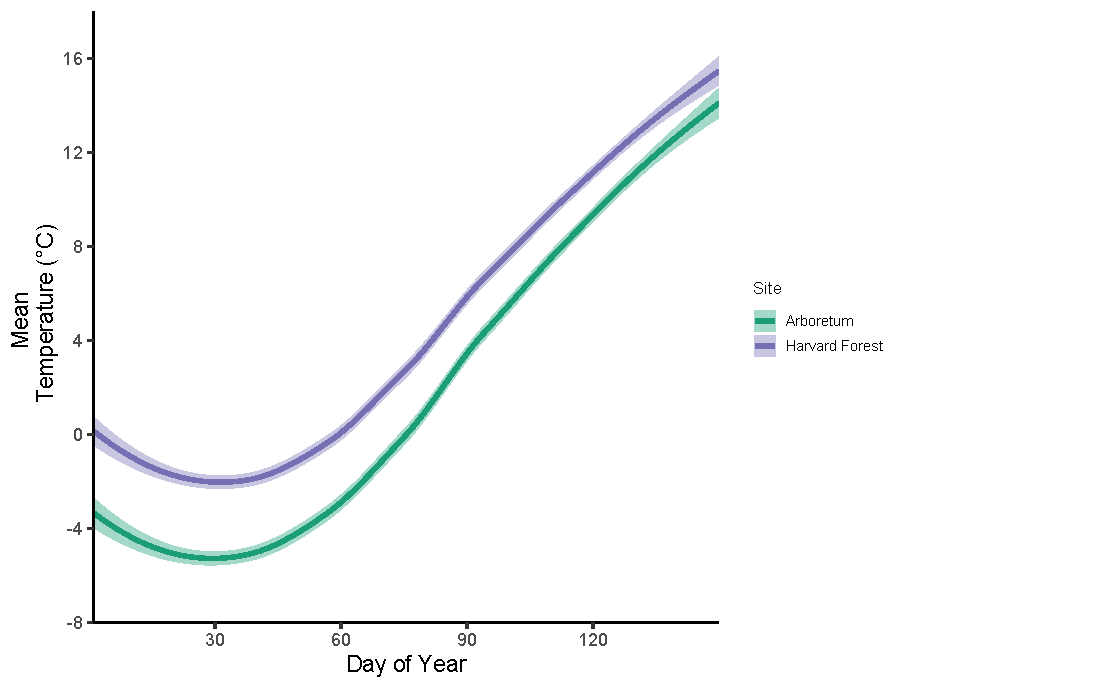
\includegraphics[width=12cm]{..//analyses/figures/climate_hfandts.pdf}
  -\caption{Smoothing spline of mean temperature with 90\% credible interval across the two sites.}\label{fig:clim}
  -\end{center}
  -\end{figure}}
  
\begin{figure}[H]
  \begin{subfigure}{.5\textwidth}
	  %\rule{\linewidth}{\dimexpr 2\linewidth+2\baselineskip+6pt}
    \caption{}
    \centering
    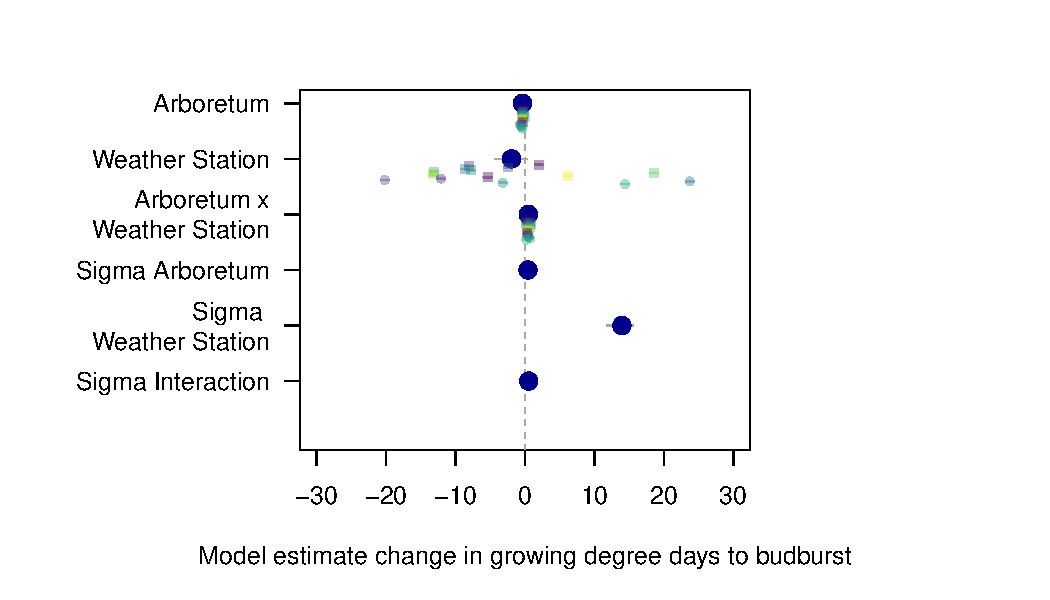
\includegraphics[height=6cm, width=10cm]{..//analyses/figures/muplot_noisyws.pdf}
    \label{fig:muplotnoisyws}
  \end{subfigure}%
    \begin{subfigure}{.5\textwidth}
	    %\rule{\linewidth}{\linewidth}
      \caption{}
      \centering
      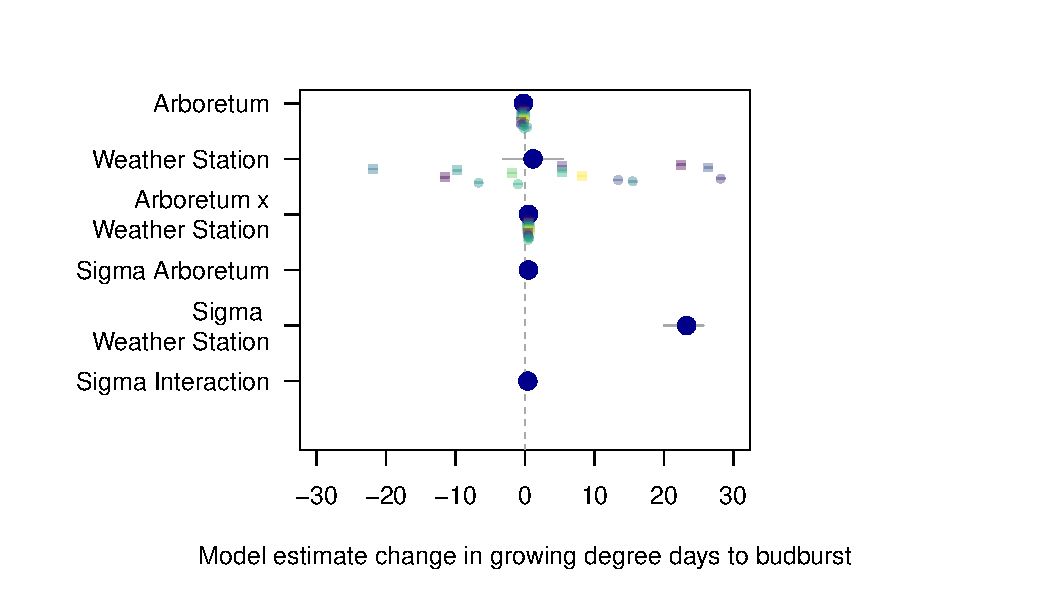
\includegraphics[height=6cm, width=10cm]{..//analyses/figures/muplot_noisyhobo.pdf}
    \label{fig:muplotnoisyhobo}
  \end{subfigure}
\caption{ We show effects of site (Arboretum as `1' or Harvard Forest as `0') and climate data method (weather station data as `1' or hobo logger data as `0') on simulated growing degree days (GDDs) until budburst using simulated data (a) with less accurate weather station data and (b) with less accurate hobo logger data. More positive values indicate more GDDs are required for budburst whereas more negative values suggest fewer GDDs are required. Dots and lines show means and 50\% uncertainty intervals. See Tables XX, XX and XX for full model outputs.}
\label{fig:simsmus}
\end{figure}


\begin{figure}[H]
  \begin{subfigure}{.5\textwidth}
	  %\rule{\linewidth}{\dimexpr 2\linewidth+2\baselineskip+6pt}
    \caption{}
    \centering
    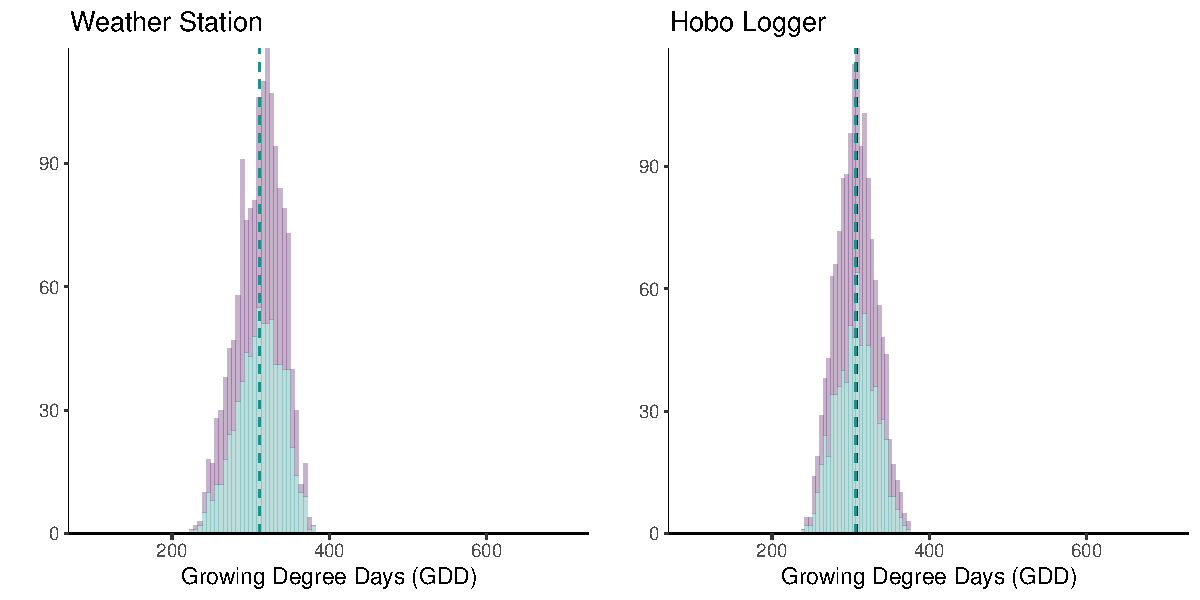
\includegraphics[height=6cm, width=10cm]{..//analyses/figures/gdd_methods_noisyws.pdf}
    \label{fig:gddnoisyws}
    \end{subfigure}
  \begin{subfigure}{.5\textwidth}
	    %\rule{\linewidth}{\linewidth}
      \caption{}
      \centering
      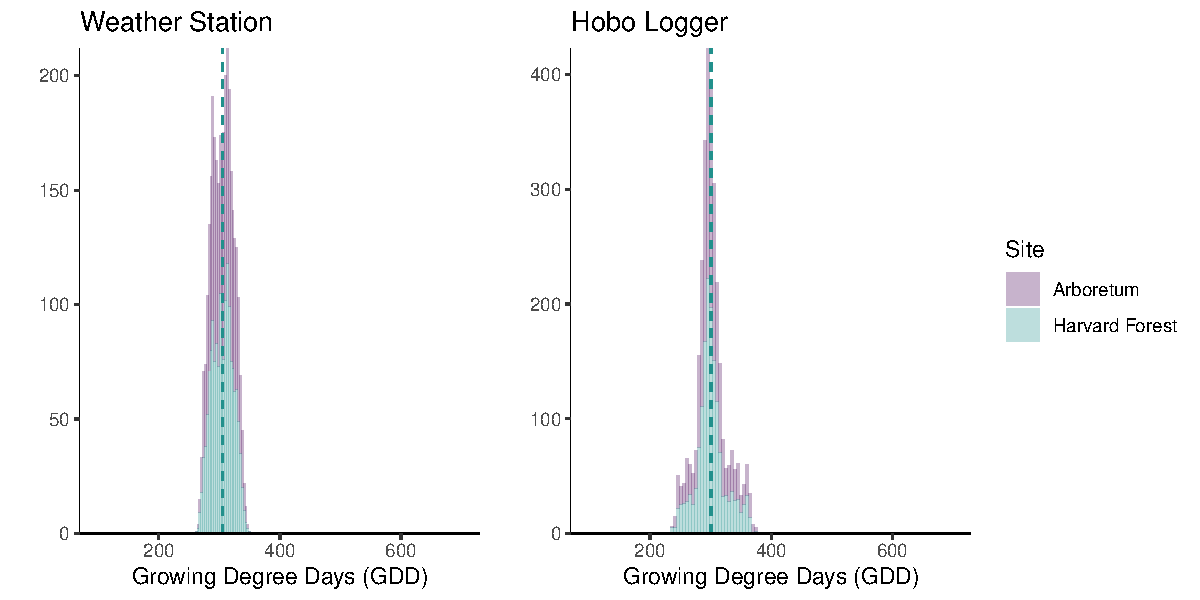
\includegraphics[height=6cm, width=10cm]{..//analyses/figures/gdd_methods_noisyhobo.pdf}
    \label{fig:gddnoisyhobo}
    \end{subfigure}
\caption{ Using simulated data with (a) less accurate weather station data and (b) less accurate hobo logger data, we show histograms of climate data at the Arboretum and Harvard Forest using weather station data and hobo logger data.}
\label{fig:climhists}
\end{figure}

\begin{figure}
  \begin{subfigure}{.5\linewidth}
	  %\rule{\linewidth}{\dimexpr 2\linewidth+2\baselineskip+6pt}
    \caption{}
      \centering
      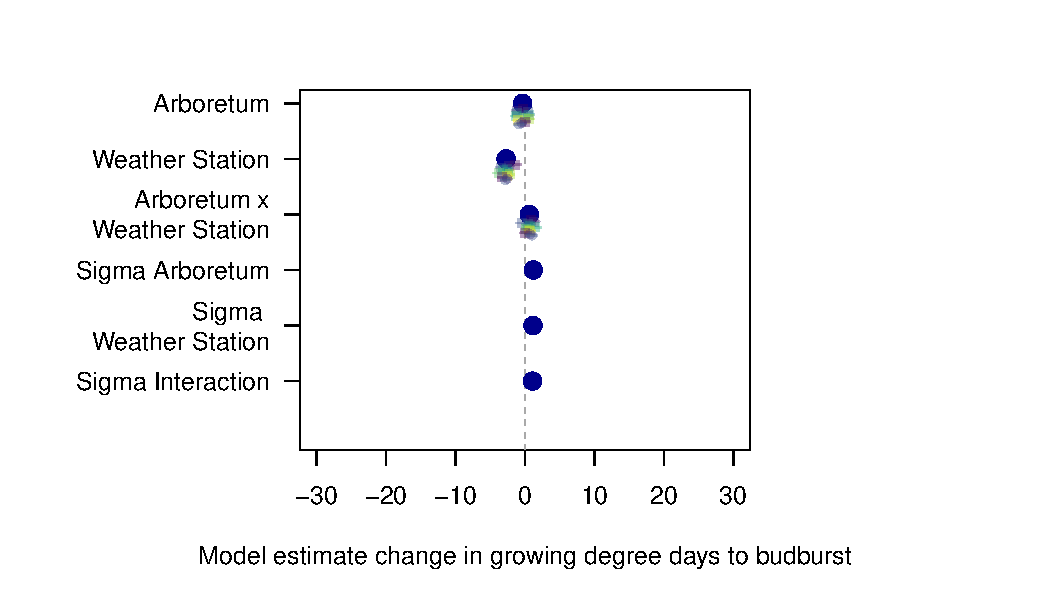
\includegraphics[height=7cm, width=11cm]{..//analyses/figures/muplot_micros.pdf}
      \label{fig:muplotmicros}
  \end{subfigure}%
    \begin{subfigure}{.5\linewidth}
	    %\rule{\linewidth}{\linewidth}
      \caption{}
      \centering
      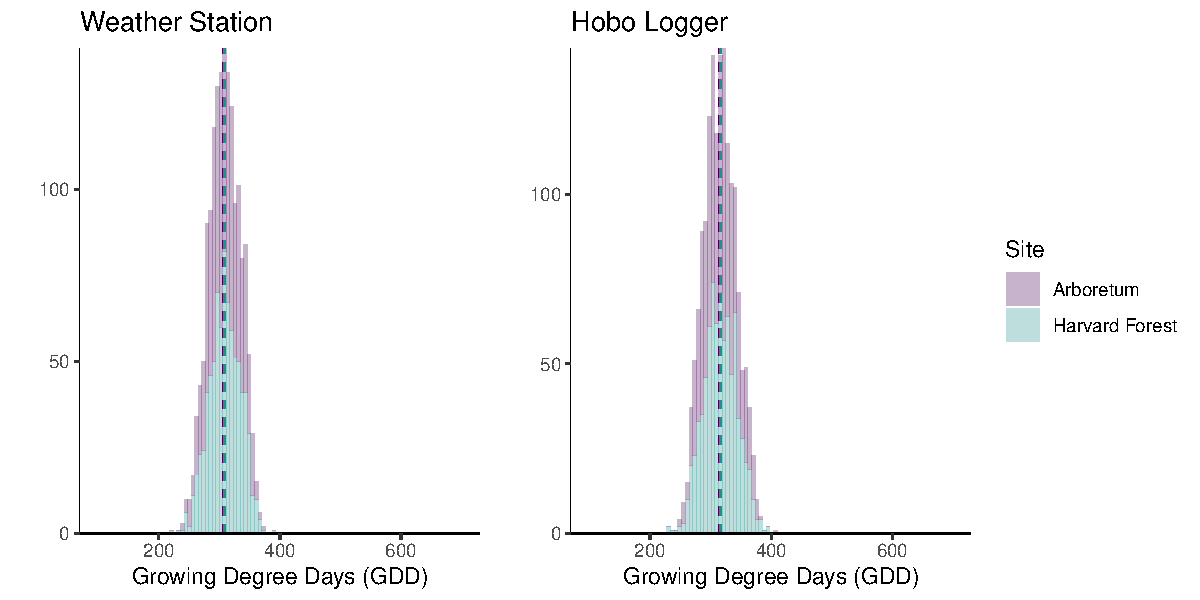
\includegraphics[height=4cm, width=8cm]{..//analyses/figures/gdd_methods_micros.pdf}
    \label{fig:gddmicros}
  \end{subfigure}\\[1ex]
\caption{ Using simulations data with microclimatic effects at both sites, we show (a) histograms of climate data at the Arboretum and Harvard Forest using weather station data and hobo logger data. (b) Histograms of GDDs at the Arboretum and Harvard Forest using weather station data and hobo logger data. (c) Effects of site (Arboretum is `1' and Harvard Forest is `0') and climate data method (weather station data as `1' or hobo logger data as `0') on simulated growing degree days (GDDs) until budburst using noisy weather station data. More positive values indicate more GDDs are required for budburst whereas more negative values suggest fewer GDDs are required. Dots and lines show means and 50\% uncertainty intervals. See Table XX for full model output.}
\label{fig:micros}
\end{figure}

\begin{figure}
  \begin{subfigure}{.5\linewidth}
	  %\rule{\linewidth}{\dimexpr 2\linewidth+2\baselineskip+6pt}
    \caption{}
      \centering
      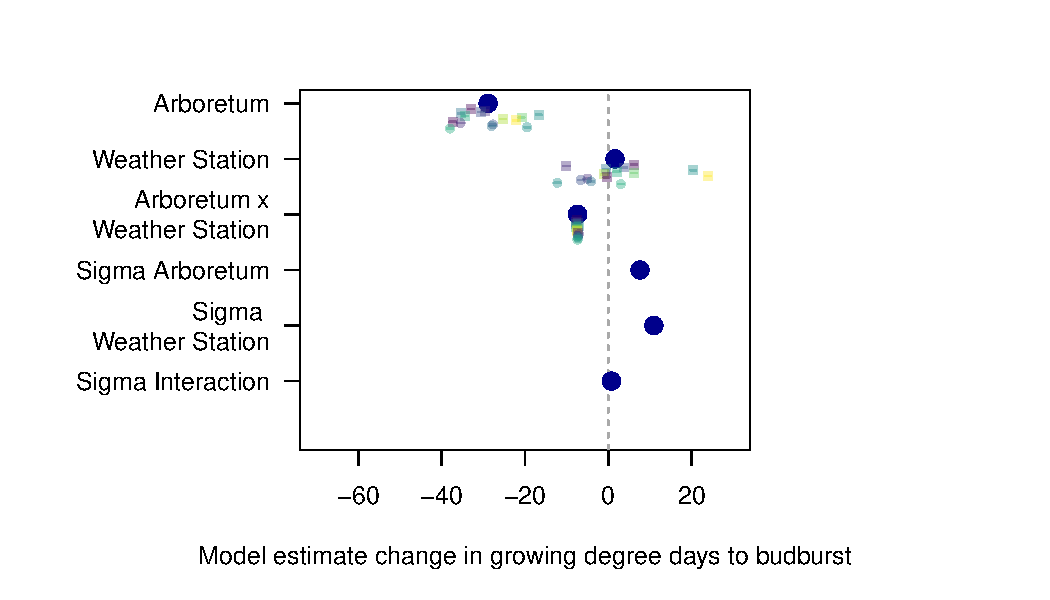
\includegraphics[height=7cm, width=11cm]{..//analyses/figures/muplot_urbws.pdf}
      \label{fig:muploturbanws}
  \end{subfigure}%
    \begin{subfigure}{.5\linewidth}
	    %\rule{\linewidth}{\linewidth}
      \caption{}
      \centering
      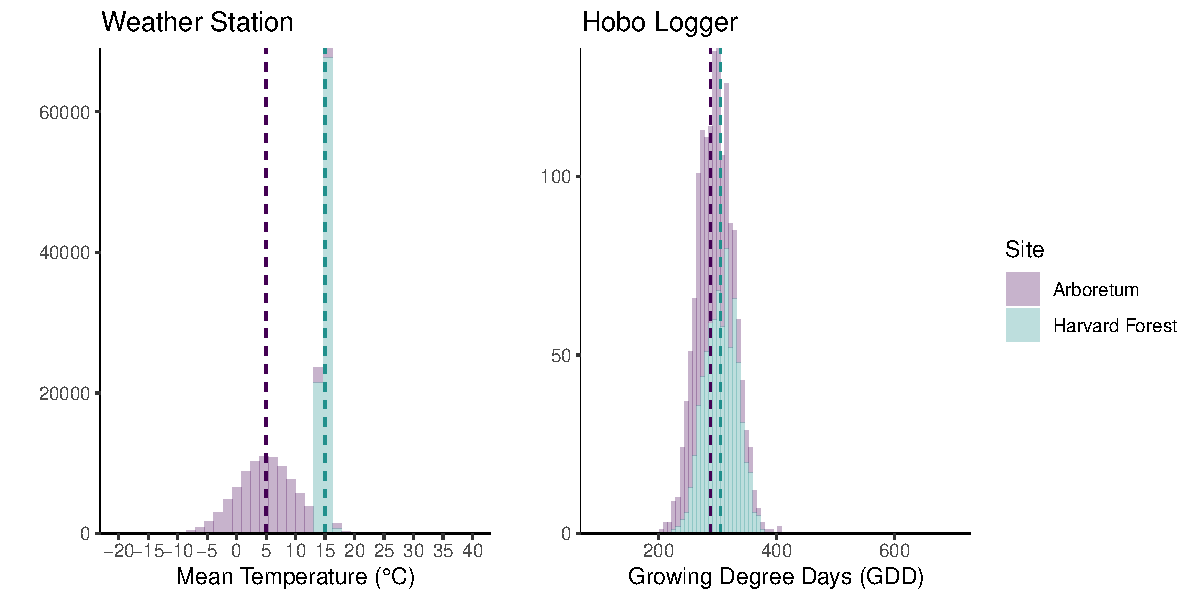
\includegraphics[height=4cm, width=8cm]{..//analyses/figures/gdd_methods_urbanws.pdf}
    \label{fig:gddurbanws}
  \end{subfigure}
\caption{ Using simulated data with the Arboretum hobo loggers recording warmer tempertures and the Harvard Forest weather station recording warmer temperatures, we show (a) histograms of climate data at the Arboretum and Harvard Forest using weather station data and hobo logger data. (b) Histograms of GDDs at the Arboretum and Harvard Forest using weather station data and hobo logger data. (c) Effects of site (Arboretum is `1' and Harvard Forest is `0') and climate data method (weather station data as `1' or hobo logger data as `0') on simulated growing degree days (GDDs) until budburst using noisy weather station data. More positive values indicate more GDDs are required for budburst whereas more negative values suggest fewer GDDs are required. Dots and lines show means and 50\% uncertainty intervals. See Table XX for full model output.}
\label{fig:urbanws}
\end{figure}

\begin{figure}
  \begin{subfigure}{.5\linewidth}
	  %\rule{\linewidth}{\dimexpr 2\linewidth+2\baselineskip+6pt}
    \caption{}
    \centering
    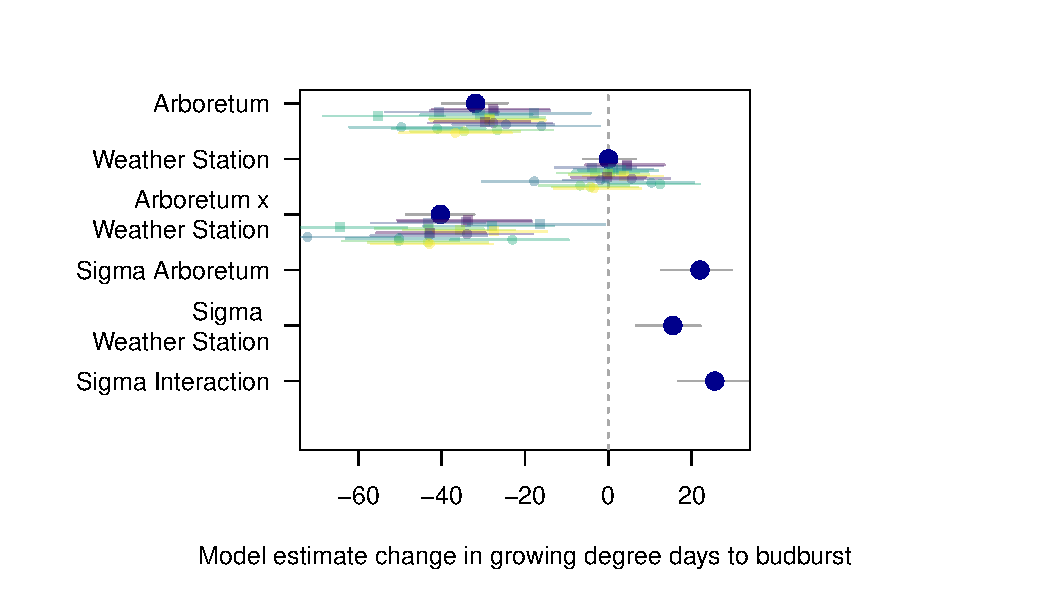
\includegraphics[height=7cm, width=11cm]{..//analyses/figures/muplot_urban_real.pdf}
    \label{fig:muplotreal}
  \end{subfigure}%
    \begin{subfigure}{.5\linewidth}
	    %\rule{\linewidth}{\linewidth}
      \caption{}
      \centering
      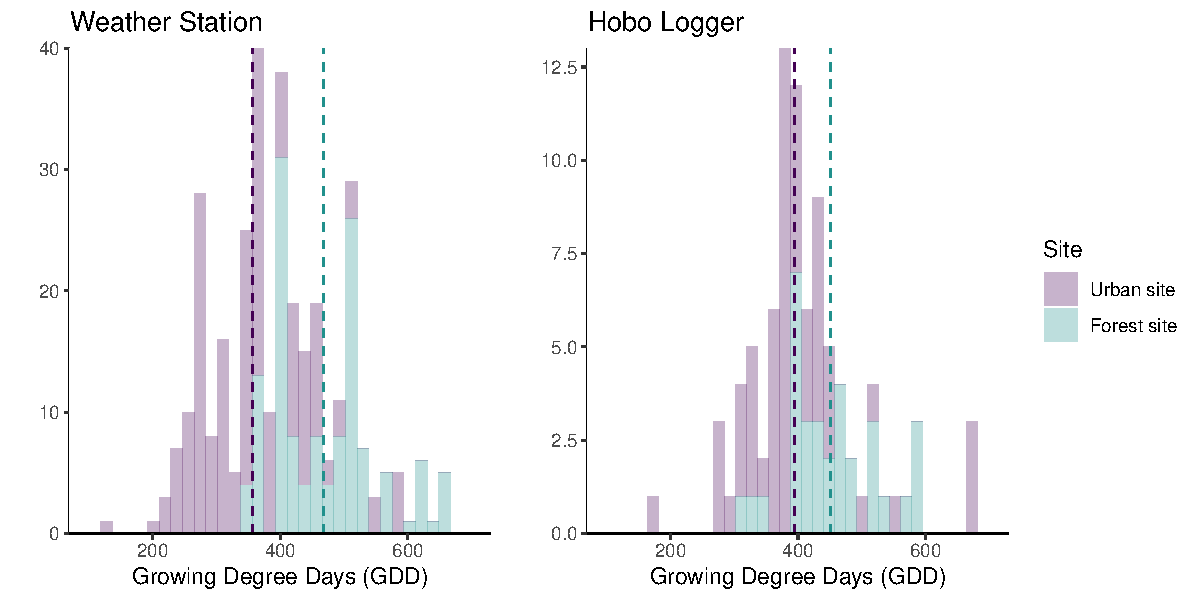
\includegraphics[height=4cm, width=8cm]{..//analyses/figures/gdd_methods_real.pdf}
    \label{fig:gddreal}
  \end{subfigure}\\[1ex]
\caption{ Using real data, we show (a) Effects of site (Arboretum is `1' and Harvard Forest is `0') and climate data method (weather station data as `1' or hobo logger data as `0') on simulated growing degree days (GDDs) until budburst using noisy weather station data. More positive values indicate more GDDs are required for budburst whereas more negative values suggest fewer GDDs are required. Dots and lines show means and 50\% uncertainty intervals. See Table XX for full model output. (b) Histograms of GDDs at the Arboretum and Harvard Forest using weather station data and hobo logger data. (c) }
\label{fig:real}
\end{figure}

\begin{figure}
  \begin{subfigure}{\linewidth}
	  %\rule{\linewidth}{\dimexpr 2\linewidth+2\baselineskip+6pt}
    \caption{}
    \centering
    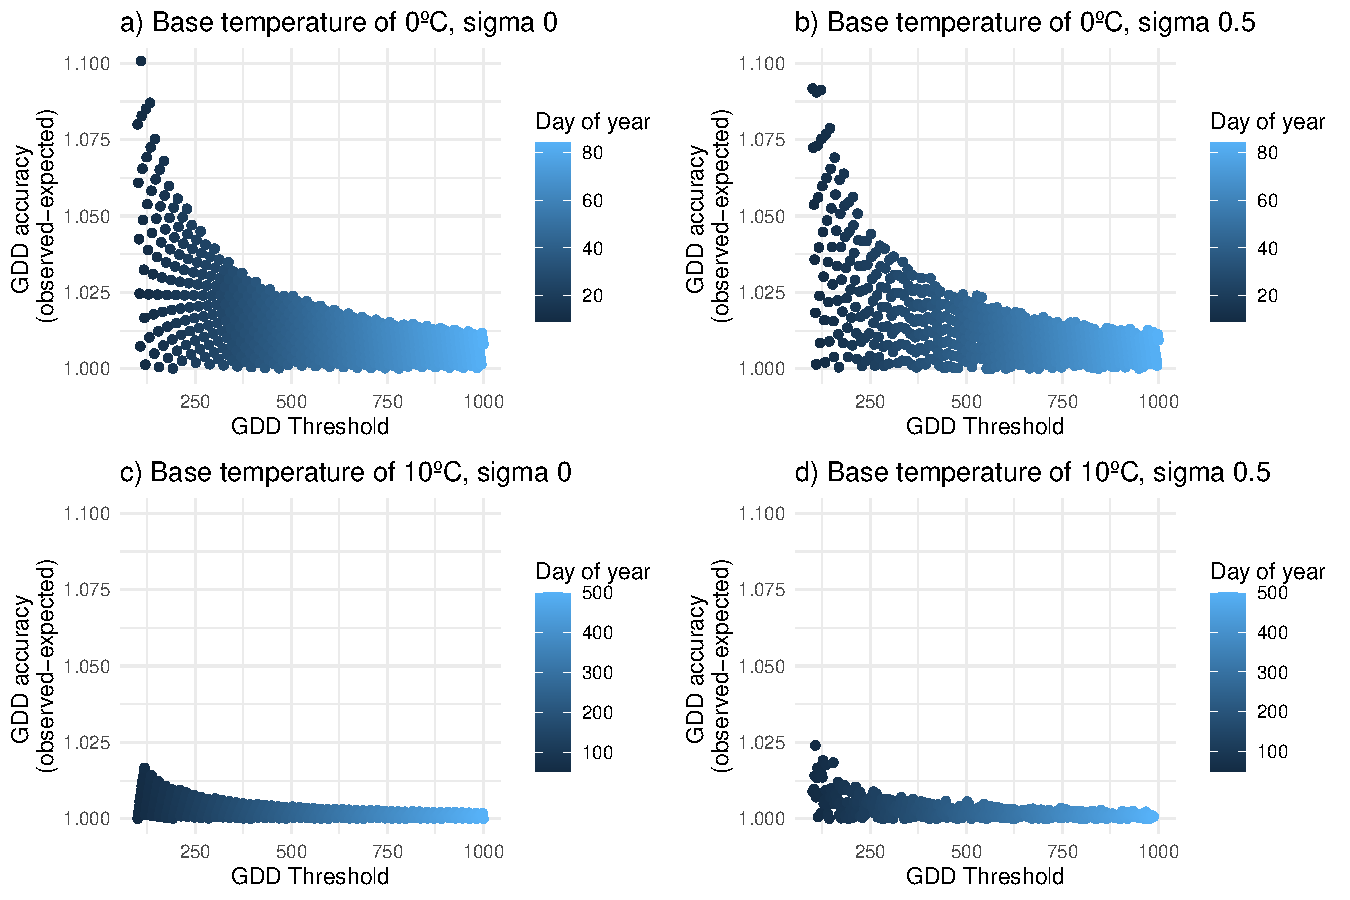
\includegraphics[height=13cm, width=14cm]{..//analyses/figures/gddratio_basetemp.pdf}
    \label{fig:forecasting}
    \end{subfigure}
  \begin{subfigure}{\linewidth}
	    %\rule{\linewidth}{\linewidth}
	    \caption{}
      \centering
      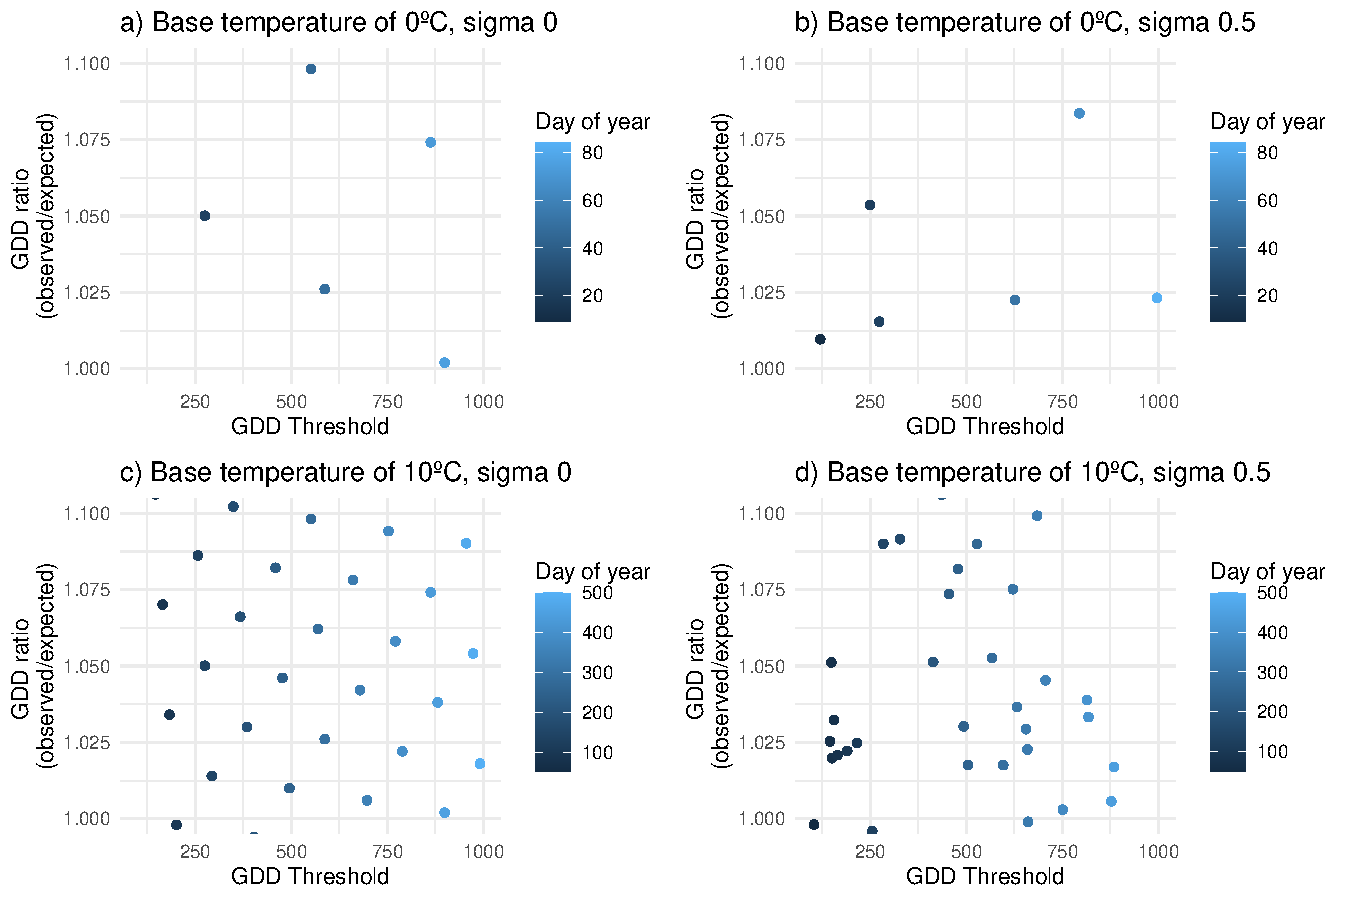
\includegraphics[height=13cm, width=14cm]{..//analyses/figures/gddaccuracy_basetemp.pdf}
      \label{fig:slopes}
  \end{subfigure}
\caption{To discuss more at our next meeting...}
\label{fig:forecasts}
\end{figure}

  
  

\end{document}
